\chapter{Anforderungen}
\section{Benutzer und Personas}
Die Benutzer der Project Helin Plattform teilen sich in drei Gruppen auf, welche in dieser Arbeit berücksichtigt werden. Die Gruppen werden nach der primären Funktion unterschieden.
\begin{itemize}
	\item{\textbf{Kunde:} Der Kunde möchte Produkte und Dienstleistungen nutzen, welche von Drohnen erbracht werden können. Beispielsweise die Bestellung eines Getränks und sofortige Lieferung an seine Position.}
	\item{\textbf{Administrator:} Administratoren verwenden die Project Helin Plattform um eine Flotte von Drohnen zu verwalten. Sie nutzen dazu die Webseite der Plattform und definieren, wo ihre Drohnen fliegen dürfen und welche Produkte und Services wo angeboten werden.}
	\item{\textbf{Drone-Operator:} Der Drone-Operator kümmert sich primär um die Drone und verwendet dafür die Onboard-App um die Drohne einem Organisationsinventar hinzuzufügen.}
\end{itemize}

Bei den Personas handelt es sich um fiktive Personen.
\subsection{Persona Diego: Kunde}
\begin{figure}[h]
\centering
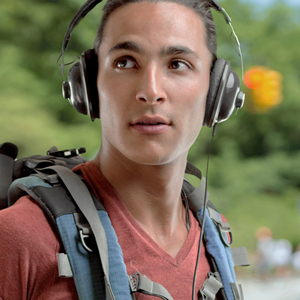
\includegraphics[width=0.35\textwidth]{images/persona-diego.jpg}
\caption{Persona Diego: Freie Lizenz; Quelle 
\protect\url{http://blog.placeit.net/free-avatar-pack/}}
\label{fig:diego}
\end{figure}
Diego ist \textbf{23 Jahre alt} wohnt in einer WG in Uster.
Diego hat eine Informatik-Lehre mit BMS abgeschlossen und ist auf der Suche nach einer neuen beruflichen oder schulischen Herausforderung.
\paragraph{Technisches Verhalten}
Arbeitet täglich acht Stunden mit dem PC. Nutzt gerne neue Technologien. Besitzt ein Android-Smartphone der neusten Generation. Die Android Updates macht er immer sofort. Interessiert sich für neue Technologien und sieht sich regelmässig Kickstarter Projekte an.
\paragraph{Ziele}
Möchte sich weiterbilden und neue Herausforderungen finden. Möchte neue Technologien entdecken und einsetzen.
\paragraph{Szenario}
Diego möchte an einem Openair ein kühles Getränk für sich und seine Freunde bestellen, er hat auf einem Plakat vor Ort gesehen, dass ein Drohnen-Lieferservice existiert und möchte aufgrund seines technischen Interesses den Dienst in Anspruch nehmen.
\subsection{Persona Carmen: Administratoren}
\begin{figure}[h]
\centering
	
\includegraphics[width=.35\textwidth]{images/persona-stefanie.jpg}
	\caption{Persona Stefanie: Freie Lizenz; Quelle
	 \protect\url{http://blog.placeit.net/free-avatar-pack/}}
	\label{fig:stefanie}
\end{figure}
Carmen ist \textbf{35 Jahre alt} und lebt alleine in Zürich.
Sie unternimmt viel mit Freunden und reist gerne. Sie ist auf dem Land aufgewachsen und wohnt jetzt in Zürich.
Carmen arbeitet bei einer Eventagentur und hat eine Ausbildung als Eventmanagerin abgeschlossen.

\paragraph{Technisches Verhalten}
Sie nutzt den PC täglich bei der Arbeit, vor allem Planungstools und das E-Mail-Programm. Ausserdem ist sie zu Recherchezwecken viel im Internet unterwegs. Sie nutzt Chrome als Browser im Geschäft. Sie besitzt ein Samsung Galaxy S4, dass sie schon seit einigen Jahren verwendet. Zuhause hat sie keinen PC.
\paragraph{Kommunikationsverhalten}
Sie kommuniziert geschäftlich hauptsächlich per E-Mail. Mit Freunden unterhält sie sich oft über WhatsApp.
\paragraph{Ziele}
Sie möchte mit neuen und innovativen Ideen Events für Besucher spannender gestalten.

\subsection{Persona Ricardo: Drone Operator}
\begin{figure}[h]
\centering
	
\includegraphics[width=.35\textwidth]{images/persona-ricardo.jpg}
	\caption{Persona Ricardo: Freie Lizenz; Quelle
	 \protect\url{http://blog.placeit.net/free-avatar-pack/}}
	\label{fig:ricardo}
\end{figure}
Ricardo ist 26 Jahre alt und wohnhaft in Wetzikon. Der ausgebildete Schlosser hat zur Zeit keinen festen Job. Er lebt das Leben von Tag zu Tag und geniest es keine festen Verpflichtungen zu haben.
\paragraph{Technisches Verhalten}
Er nutzt den PC selten, vorallem aber zum Surfen im Internet. Als Mobiltelefon besitzt er ein altes Telefon mit Android. Er möchte sich auch kein neues Gerät kaufen, da er ausser Whatsapp und der Taschenlampe das Gerät sowieso nicht verwendet.
\paragraph{Kommunikationsverhalten}
Er verwendet hautpsächlich Email und sein Mobiltelefon zur Kommunikation. Mit Freunden unterhält sie sich auch oft über WhatsApp.
\paragraph{Ziele}
Ricardo möchte gerne am Openair etwas Geld dazu verdienen und ohne grosse Einarbeitungszeit den Anforderungen der Eventtechnikfirma genügen.
\newpage
\section{Funktionale Anforderungen (User Stories)}

Die funktionalen Anforderungen leiten sich aus der Aufgabenstellung, sowie den mit dem Betreuer diskutierten Ideen ab.

\subsection{Administrator}
\begin{itemize}
\item Als Administrator möchte ich auf der Webseite einen Account erstellen können.
\item Als Administrator möchte ich meine Organisation verwalten können (CRU). (zusätzlich, siehe unten)
\item Als Administrator möchte ich neue Administratoren hinzufügen und entfernen können. (zusätzlich)
\item Als Administrator möchte ich ein Projekt erfassen können.
\item Als Administrator möchte ich auf eine Drohne dem Projekt hinzufügen können.
\item Als Administrator möchte ich alle Drohnen verwalten können (RUD).
\item Als Administrator möchte ich Produkte verwalten können (CRUD).
\item Als Administrator möchte ich Produkte einem Projekt hinzufügen können (zusätzlich)
\item Als Administrator möchte ich Services (zum Beispiel Drone Selfies) verwalten können (CRUD). (optional)
\item Als Administrator möchte ich Flug-, Lade- und Abwurfzonen verwalten können.
\item Als Administrator möchte ich Bestellungen verwalten können (CRUD) (teilweise ausgeschlossen).
\item Als Administrator möchte ich Telemetriedaten der Drohne, sowie die berechnete Route vor, nach, und während der Auslieferung einer Bestellung ansehen können.
\item Als Administrator möchte ich Bestellungen abbrechen können. (ausgeschlossen)
\end{itemize}

\subsection{Kunde}
\begin{itemize}
	\item Als Kunde möchte ich eine App aus dem Google Play Store herunterladen können um diese verwenden zu können.
	\item Als Kunde möchte ich die App nutzen ohne mich anmelden zu müssen.
	\item Als Kunde möchte ich in der App, aus einer Liste von Produkten und Services, eine Auswahl treffen können.
	\item Als Kunde möchte ich nur Produkte und Services sehen, die in meiner Umgebung angeboten werden. (zusätzlich)
	\item Als Kunde möchte ich eine Bestellung tätigen können.
	\item Als Kunde möchte ich die bestellte Ware direkt bezahlen können. (optional)
	\item Als Kunde möchte ich auf der Karte des Smartphones die Bewegung der Drohne verfolgen können um abzuschätzen wann meine Lieferung eintrifft.
	\item Als Kunde möchte ich eine Bestellung stornieren können (ausgeschlossen).
\end{itemize}

\subsection{Drone-Operator}
\begin{itemize}
	\item Als Drone-Operator möchte ich eine Android App mit Hilfe der heruntergeladenen \Gls{APK} installieren können.
	\item Als Drone-Operator muss ich das die Drohne beim Server registrieren können.
	\item Als Drone-Operator muss ich das die Drohne zu einer Organisation hinzufügen können.
	\item Als Drone-Operator muss ich das \Gls{OTG}-fähige Smartphone an einen MAV-Link kompatiblen Flight-Controller über USB anschliessen können.
	\item Als Drone-Operator muss ich eine Verbindung zwischen App und Server über das Internet herstellen könnnen.
	\item Als Drone-Operator muss ich eine Verbindung zwischen App und Flight-Controller herstellen können.
	\item Als Drone-Operator möchte ich den aktuellen Zustand der Verbindungen zur Drohne und zum Server sehen.
	\item Als Drone-Operator möchte ich den aktuellen Status des \Gls{Flight-Controller}, beispielsweise GPS und Batteriespannung sehen.
	\item Als Drone-Operator möchte ich eine Liste von Produkten angezeigt bekommen, die für die aktuelle Mission geladen werden müssen.
	\item Als Drone-Operator möchte ich eine Mission annehmen oder ablehnen können um eine Drohne bei Problemen austauschen zu können.
	\item Als Drone-Operator möchte ich die Beladung einer Drohne bestätigen können.
	\item Als Drone-Operator erhalte ich ein visuelles und akustisches Countdown-Signal bevor die Drohne startet.
	\item Als Drone-Operator möchte ich den Start der Drohne während des Countdowns verhindern können.
\end{itemize}

\subsection{Nachträglich ausgeschlossene Anforderungen}

\subsubsection{Bestellung löschen und ändern}
Gemäss den anfänglichen Anforderungen sollte der Administrator die Möglichkeit haben eine Bestellung zu bearbeiten (CRUD). Dies wurde reduziert auf das Ansehen von Bestellungen (R). Nur ein Kunde sollte die Möglichkeit haben eine Bestellung zu löschen, da auch er sie erstellt hat. Ausserdem muss es auch dort Einschränkungen geben, da eine bezahlte Bestellung unter keinen Umständen gelöscht werden sollte.


\subsubsection{Mission abbrechen}

Das Abbrechen einer Mission wurde aus dem Scope entfernt, da sich einerseits Fragen über den sinvollen Einsatz eines solchen Features stellten und dafür andere Tasks wie das Payment priorisiert werden konnten.

\subsection{Nachträglich hinzugefügte Anforderungen}

\subsubsection{Verwalten von Organisationen}

Um die Applikation Multi-Tenant-Fähig zu machen, wurden Organisationen eingefügt. Diese trennen verschiedene Kunden komplett ab und ermöglichen den Einsatz als Software as a Service.

\subsubsection{Administratoren Hinzufügen und Entfernen}

Um Organisationen nutzbar zu machen, musste es auch möglich sein zusätzliche Administratoren zu einer Firma hinzuzufügen und wieder zu entfernen.

\subsubsection{Produkte einem Projekt hinzüfen}

Damit Organisationen nur einmal ihre Produkte erfassen müssen und diese dann für verschiedene Projekte (z.B. Events) verwenden können, gehören Produkte immer zu einer Organisation und zu beliebig vielen Projekten. (siehe Abb. \ref{fig:domain-model})

\subsubsection{Nur verfügbare Produkte anzeigen}

Damit ein Kunde nur die für ihn relevanten Angebote sieht, werden nur Produkte und Services angezeigt, die an seiner Position verfügbar sind.

\newpage
\section{Nichtfunktionale Anforderungen}
\subsection{Verbindungsabbruch}
\begin{tabular}{|p{.25\textwidth}|p{.75\textwidth}|} \hline
	Synopsis & Verbindungsabbruch der Onboard App zum Server soll keine negativen Auswirkungen auf die Mission haben.  \\ \hline
		
	Messbarkeit & Nach dem Start der Mission schliesst die Drohne, auch ohne Verbindung zum Server, die Mission ab. \\ \hline
\end{tabular}

\subsection{Sicherheit im Mittelpunkt}
\begin{tabular}{|p{.25\textwidth}|p{.75\textwidth}|} \hline
	Synopsis & Eine Drohne führt vor dem Freigeben der Motoren (Arming) einen Check durch, der prüft ob alle nötigen Voraussetzungen für einen Start erfüllt sind. Ausserdem müssen vor einem Start ebenfalls Voraussetzungen der Mission erfüllt sein, beispielsweise muss der Drone-Operator den Start freigeben. Sollte eine dieser Vorraussetzungen nicht erfüllt sein, darf die Drohne nicht starten.  \\ \hline
	
	Messbarkeit & Drohne startet nicht, falls der Pre-Flight-Check des Autopiloten nicht erfolgreich war oder Voraussetzungen für die aktuelle Mission nicht erfüllt sind. \\ \hline
\end{tabular}
\subsection{Verbindungswiederherstellung}
\begin{tabular}{|p{.25\textwidth}|p{.75\textwidth}|} \hline
	Synopsis & Nach einem Verbindungsabbruch zwischen dem Server und der Onboard App soll die Verbindung wiederhergestellt werden sobald wieder Internet verfügbar ist. \\ \hline
	
	Messbarkeit & Die Verbindung zwischen Server und App wird nach dem deaktivieren und wieder aktivieren der Internetverbindung innert 30 Sekunden wiederhergestellt.\\ \hline
\end{tabular}

\subsection{Security}
\subsubsection{Messaging-Verbindungen}
\begin{tabular}{|p{.25\textwidth}|p{.75\textwidth}|} \hline
	Synopsis & Es darf nicht möglich sein, dass jemand die Steuerung einer beim Server registrierten Drohne übernehmen kann.\\ \hline
	Messbarkeit & Der Übertragungskanal vom Server zur Drohne ist verschlüsselt und es können sich keine weiteren \Gls{Message-Producer} anmelden.\\ \hline
\end{tabular}

\subsubsection{HTTP-Verbindungen}
\begin{tabular}{|p{.25\textwidth}|p{.75\textwidth}|} \hline
	Synopsis & Die Verbindung zum Server von jedem Client muss verschlüsselt sein.\\ \hline
	Messbarkeit & Die Verbindung über den Webbrowser lässt nur HTTPS zu. Die Verbindung vom Customer-App zum Server läuft über HTTPS und Secure-Websockets. Die Verbindung vom Onboard-App zum Server läuft über HTTPS.\\ \hline
\end{tabular}

\section{Domain-Model}
Aus den funktionalen Anforderungen ergibt sich das folgende Domainmodel.
\begin{landscape}
\begin{figure}[h]
	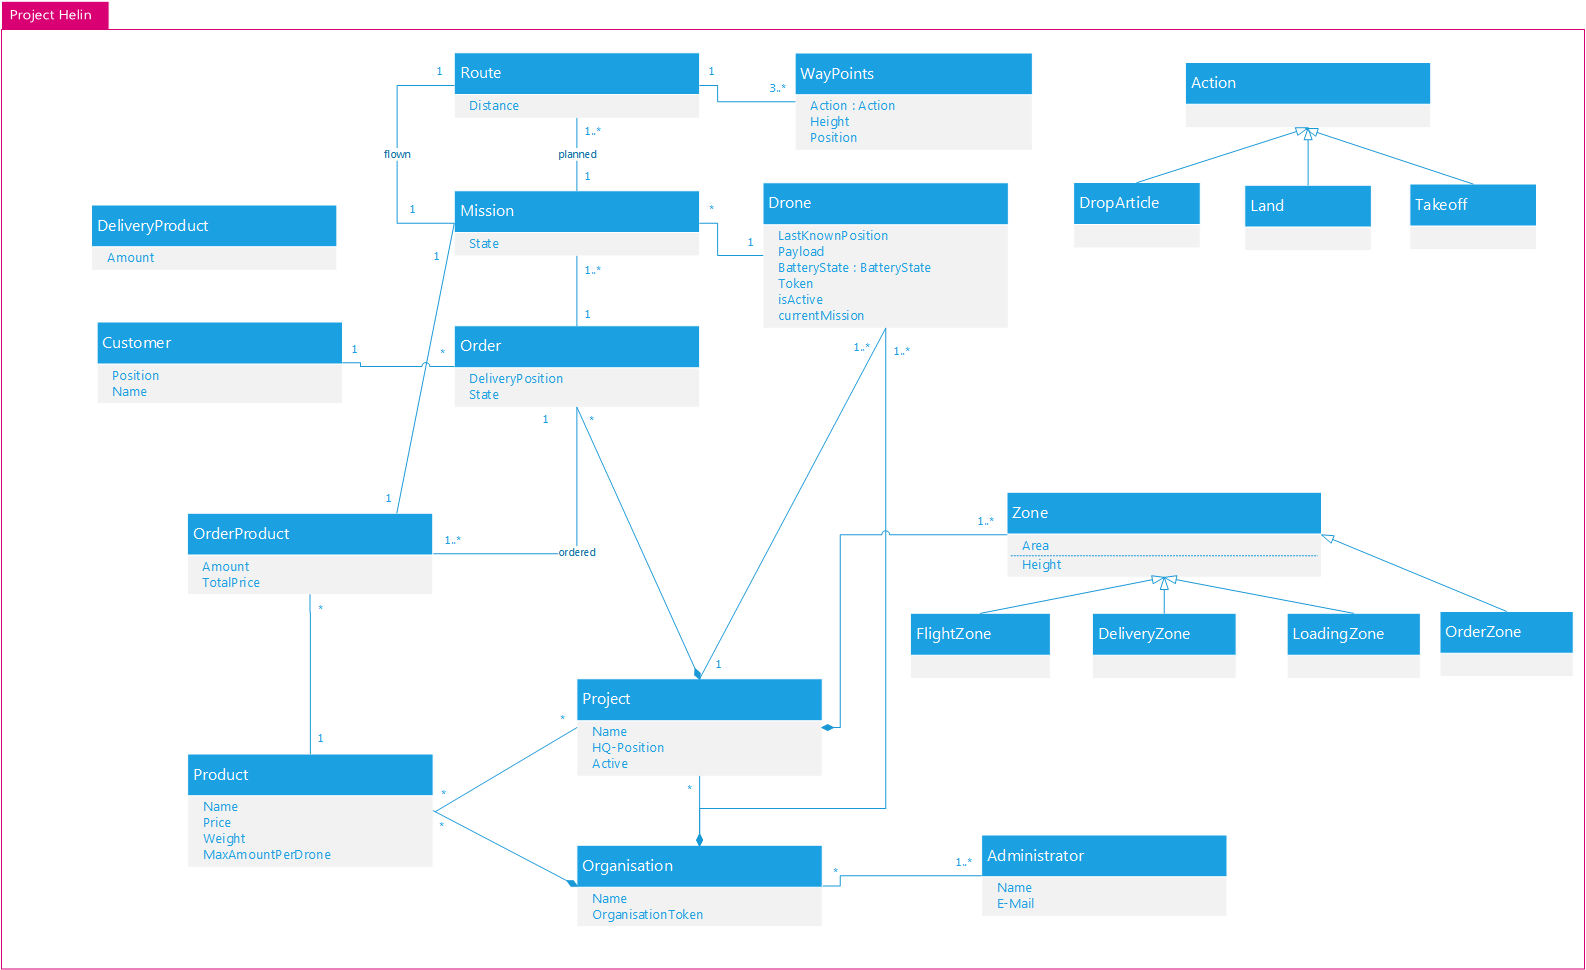
\includegraphics[width=0.75\paperheight]{images/domainmodell.png}
	\caption{Domain-Model}
	\label{fig:domain-model}
\end{figure}
\end{landscape}

